\section{Considerações Iniciais}
Este capítulo apresenta o projeto como um todo, explicando escolhas que foram 
feitas em seu desenvolvimento, tais como ferramentas e tecnologias adotadas. 
 


\section{Projeto}
Com o intuito de desenvolver um ambiente de ensino que fosse igualmente conveniente 
para professores estruturarem suas disciplinas de programação, 
tanto quanto agradável para alunos participarem de atividades, desenvolveu-se nesta monografia
 uma prova de conceito do que se envisinou poder ser esse sistema. Espera-se que, a partir 
 desta prova de conceito, atraía-se interessados pela construção de uma solução e 
 que, de forma coletiva, construa-se uma plataforma de excelência,
 por meio de colaborações em código aberto.

O professor na plataforma é capaz de criar e gerenciar exercícios, trilhas e turmas. 
Alunos se inscrevem na plataforma por meio de um \emph{login} de identidade federada, e 
ingressam nas turmas por meio de um \emph{link} específico, que é fornecido 
pelo professor nos primeiros dias de aula. 

Trilhas de exercícios são preparadas por professores, que a associam às suas turmas. 
Estas trilhas são compostas de Grupos de Exercícios Equivalentes que 
contêm exercícios de assuntos correlatos e, idealmente, de mesmo nível de dificuldade.
Para cada aluno, é sorteado um exercício de cada grupo de forma aleatória. 
Caso o aluno apresente dificuldade na resolução deste exercício, o aluno pode solicitar 
dicas relativas ao exercício, ou, em último caso, a solução do mesmo. Caso a solução 
seja requisitada, outro exercício do mesmo passo é sorteado a este aluno.

Para diminuir o escopo inicial do projeto e incentivar o estudante a se familiarizar com o ferramental 
que envolve desenvolvimento de software, escolheu-se que o desenvolvimento do código 
acontecesse localmente no computador do aluno. Para que, ainda sim, proporcionemos ao aluno 
uma boa experiência, desenvolveu-se uma interface por linha de comando, que nos referiremos a partir de agora 
por \emph{CLI} (\emph{Command Line Interface}). Por meio desta \emph{CLI},
o aluno pode fazer \emph{downloads} e submissões
dos exercícios propostos de maneira rápida e prática.

Dessa forma o sistema está dividido em três partes: uma interface gráfica, \emph{frontend}, 
em que professores e alunos possam interagir com exercícios, trilhas e turmas, uma \emph{CLI} que possibilita 
\emph{download} e submissão de exercícios, e um servidor com uma \emph{API} capaz de abstrair 
os recursos necessários por ambos os clientes. Na \fref{fig:arquitetura} apresenta-se um diagrama 
da arquitetura do sistema.

  \begin{figure}[htpb]
    \centering
    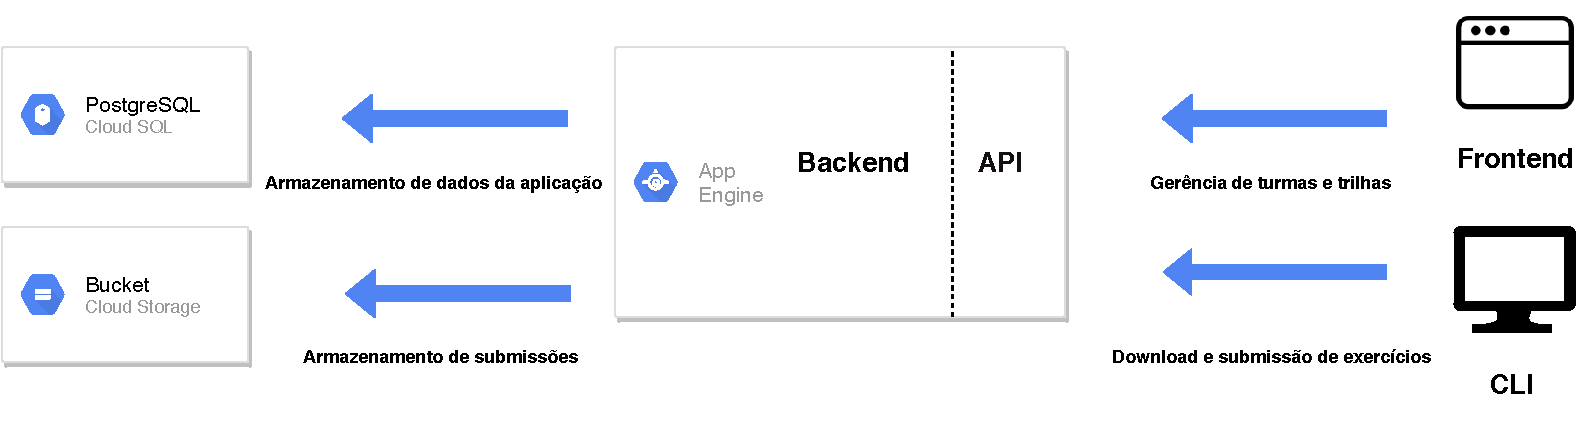
\includegraphics[width=\linewidth]{images/arquitetura.pdf}
    \caption{Diagrama que explica a arquietura do sistema \emph{Sharpener}, o qual 
    se desenvolveu uma prova de conceito.}%
    \label{fig:arquitetura}
  \end{figure}



\section{Atividades Realizadas}
\subsection{Desenvolvimento da \emph{API}}
Para o desenvolvimento da \emph{API}, escolheu-se a linguagem \emph{Python}, por sua clareza, 
e sua alta produtividade, que é crucial no processo de prototipação. Em conjunto com \emph{Python}, 
o \emph{micro framework web} \emph{Flask} também foi escolhido. Justifica-se essa escolha pela
inerente simplicidade, clareza e produtividade do \emph{framework}. 

Antes de podermos modelar recursos para a \emph{API},
estudou-se quais dados eram necessários para os casos de uso propostos. Este estudo gerou um 
\emph{MER}, modelo entidade relacional, que relacionava todas as entidades do sistema. A partir 
do diagrama gerado, criou-se ``\emph{models}'' que representavam estas entidades. A classe 
que possibilitou a criação destes \emph{models} provêm da \emph{ORM} que abstraí bancos 
relacionais chamada \hyperref[link:sqlalchemy]{\emph{SQLAlchemy}}. \hyperref[link:sqlalchemy]{\emph{SQLAlchemy}}
é uma biblioteca estável com mais de treze anos de maturidade,
mas que continua sendo a escolha padrão dos desenvolvedores.

Optou-se por utilizar \hyperref[link:postgresql]{\emph{PostgreSQL}}.
A escolha foi feita por se tratar de um sistema 
gerenciador de banco de dados relacional de código aberto e por este ser referência em 
desempenho e funcionalidades.

No mapeamento do \emph{MER}, previamente esboçado, em classes utilizou-se a biblioteca 
de visualização \hyperref[link:eralchemy]{\emph{ERAlchemy}}. \hyperref[link:eralchemy]{\emph{ERAlchemy}} é capaz de gerar 
diagramas \emph{MER} de forma automática a partir das classes modelo ou de uma conexão com o banco de dados. 
Tal ferramenta se provou excepcionalmente útil pois permitiu o desenvolvimento incremental e iterativo das 
classes modelo e garantiu que o modelo conceitual fosse implementado sem divergências. A \fref{fig:mer} mostra 
o modelo entidade relacional do sistema, gerado a partir da ferramenta.

Para que nosso sistema fosse capaz de armazenar submissões de alunos de forma confiável,  
um serviço de intervalos de  armazenamento, traduzido do inglês \emph{Bucket Storage}, se 
fez necessário. Um intervalo de armazenamento nada mais é que uma abstração de provedores 
de computação em nuvem para oferecer armazenamento de objetos. Uma das grandes vantagens associadas 
a este tipo de serviço é o baixo custo por \emph{gigabyte}, além de sua alta escalabilidade, tanto 
 um aumento no volume de dados armazenados, quanto na velocidade recuperação destes.
O provedor de computação em nuvem escolhido foi a \hyperref[link:gcp]{\emph{Google Cloud Plataform}}.


A alternativa a adotar um serviço de armazenamento por intervalos seria armazenar arquivos 
diretamente no banco de dados, o que traria um impacto na performance do mesmo, já que \emph{SGBD}s não são otimizados para
este tipo de dado. 

Modelou-se recursos seguindo o estilo arquitetural \emph{REST}. Coleções e documentos
de exercícios, turmas, tópicos, entre outros recursos foram implementados, e um 
recurso do arquétipo \emph{controller} foi necessário para prover autenticação a interface por 
meio do fluxo de concessão do código de autorização. Também disponibilizou-se uma rota para \emph{health check}, 
que permite que uma sonda externa consulte se a aplicação continua funcionando adequadamente. Caso esta não esteja, 
envia-se um sinal para que um novo container da aplicação seja iniciado e o tráfego é redirecionado a ela. 

Para que não seja necessário que professores criem um banco de exercícios do zero, um ``conector'' foi 
implementado para a plataforma \emph{exercism}, em que seus exercícios são extraídos e guardados no banco 
de dados. A implementação aborda apenas duas linguagens \emph{Python} e \emph{Rust}, mas 
pode ser facilmente estendido para outras linguagens, dado que se informe a estrutura de arquivos 
que os exercícios daquela linguagem são armazenados.

Também foi configurado uma plataforma de \emph{CI/CD} para o projeto. A toda nova versão enviada 
ao repositório remoto do sistema de controle de versões, uma tarefa rodava a ferramenta \emph{autopep8}
que checava se o código \emph{commitado} era sintaticamente válido e não seguia más práticas. 
Caso o código fosse reprovado na tarefa anterior, este não poderia ser aprovado e mesclado 
na \emph{branch} principal de desenvolvimento. Se a contribuição passar na verificação e 
depois de revisão for aceita, uma tarefa para lançamento da nova versão é disparada automaticamente, 
       que coloca uma nova versão no ar. A plataforma de \emph{CI/CD} empregada foi o 
       \hyperref[link:actions]{\emph{Github Actions}} e 
       as novas versões eram colocadas no ar através da \emph{Platform as a Service} do \emph{Google}, 
       \hyperref[link:appengine]{\emph{AppEngine}}.

\begin{sidewaysfigure}[htpb]
    \centering
    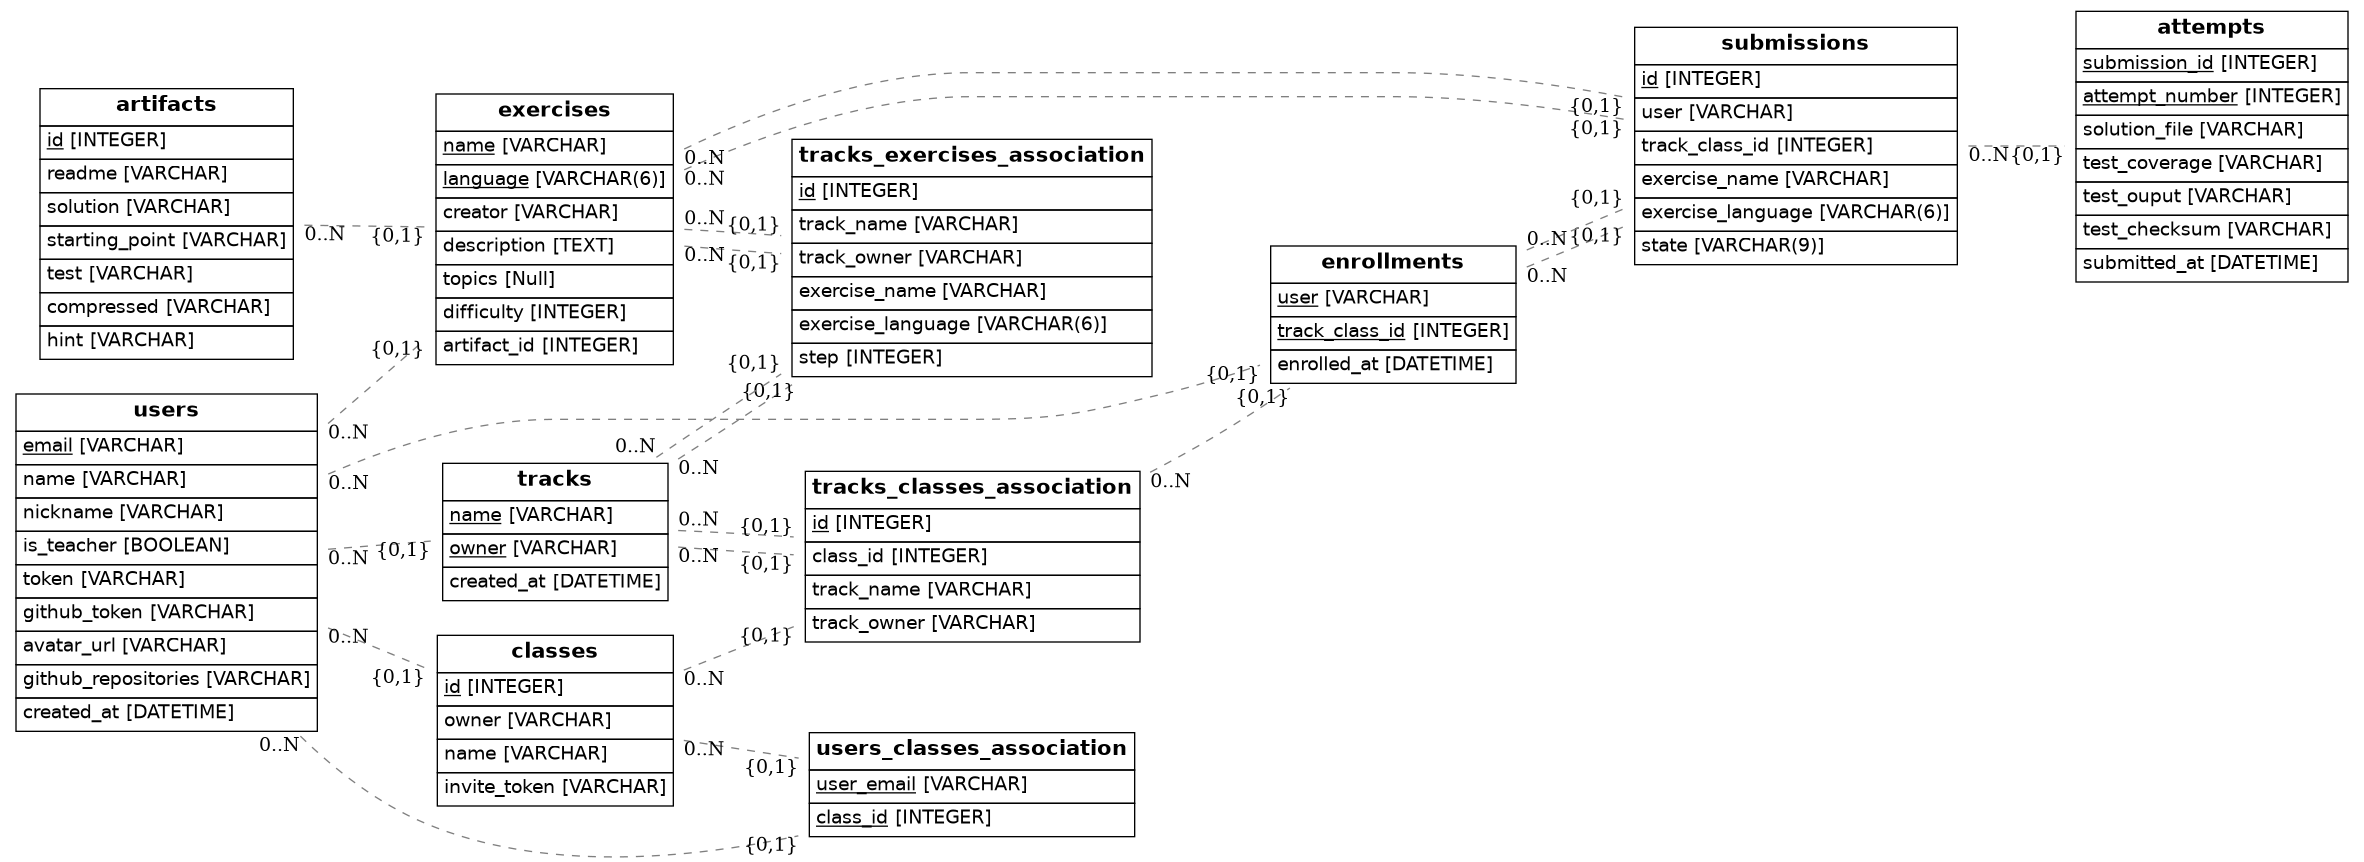
\includegraphics[width=\linewidth]{images/db_schema}
    \caption{Modelo entidade relacional gerado a partir da ferramenta \hyperref[link:eralchemy]{\emph{ERAlchemy}}.}\label{fig:mer}
\end{sidewaysfigure}


\subsection{Desenvolvimento da interface}
A interface foi desenvolvida utilizando \emph{Javascript}, \emph{CSS} e \emph{HTML}. Como 
desejávamos uma plataforma que fosse bastante interativa, uma \emph{single page application} 
foi implementada, utilizando a tecnologia \hyperref[link:react]{\emph{React}}.
Seguiu-se o \emph{design system} chamado 
\emph{Material Design} por ser bastante intuitivo para novos usuários. A biblioteca \emph{Material-UI} 
forneceu vários componentes que serviram de base para os componentes customizados. A comunicação com a 
\emph{API} foi feita utilizando o cliente \emph{HTTP} \hyperref[link:axios]{\emph{axios}} e 
os dados são persistidos numa \emph{store} local, utilizando o gerenciador de estados \emph{Redux}.


\subsection{Desenvolvimento da CLI}
O desenvolvimento da \emph{CLI} foi feito na linguagem \emph{Rust}, utilizando 
a biblioteca \emph{StructOpt}. \emph{StructOpt} é uma biblioteca que permite construção 
de interfaces por linhas de comando a partir da anotação de macros em \emph{structs} ou 
\emph{enums}. Com uma simples anotação ganha-se um \emph{parser} dos comandos e mensagens 
que instruem o usuário como utilizar sua \emph{CLI}.
 
 Aceitam-se três comandos na \emph{CLI}, ``\emph{download}'' que a partir de um identificador busca 
 o exercício proposto, \emph{submit} que manda uma tentiva de solução do problema ao servidor e 
 \emph{config}, necessário que seja executado, ao menos uma vez, com uma chave que identifica 
 qual aluno está utilizando o programa.

\section{Resultados}
A \fref{fig:login} mostra a página inicial da interface \emph{web} da ferramenta \emph{Sharpener}.
O \emph{login} do usuário é feito por contas previamente cadastradas na plataforma \emph{Github},
por meio fluxo de código de acesso. O professor quando logado, será direcionado a página 
de suas turmas, retratada na \fref{fig:turmas}, em que poderá gerenciá-las. Nesta página 
o professor também inscreve suas turmas em trilhas previamente criadas, como podemos 
observar em \fref{fig:enroll_track}. 

Pode-se acessar a página que possibilita a criação de trilhas 
através do menu lateral, que o leva a página retratada pela \fref{fig:track}. Nesta página 
pode-se criar novas trilhas como mostrado na \fref{fig:add_track1}. Uma trilha é composta por 
vários ``passos'', que são os \emph{clusters} de exercícios discutidos anteriormente. 
Ao clicar no botão de adicionar exercícios, surge um novo componente em que pode-se buscar 
e selecionar exercícios que farão parte daquele passo, conforme podemos observar em 
\fref{fig:add_track4}. Sabemos que a elaboração de exercícios é uma tarefa que toma 
muito tempo, portanto na página de exercícios, retratada pela \fref{fig:exercicios},
professores podem buscar por novos exercícios,  que foram criados por outros professores 
ou extraídos de alguma repositório público.


\section{Dificuldades e Limitações}
Encontraram-se duas grandes dificuldade na condução deste trabalho. 
A primeira delas foi a orquestração de diferentes tecnologias e partes do sistema. Houve um 
alto custo associado a dominar, utilizar e integrar diferentes linguagens, \emph{frameworks} 
e serviços. Ao longo do desenvolvimento deste projeto, percebeu-se que o escopo do projeto 
abordado foi inadequado para desenvolvimento no decorrer de um semestre.

Apesar, desde a concepção do projeto, o desenvolvimento proposto era de apenas uma prova 
de conceito de um sistema, esperava-se que, ao final da disciplina, um protótipo já adequado 
para testes em salas de aula fosse alcançado. Infelizmente, tal expectativa não foi cumprida.  
Apesar de uma parte significativa do sistema ter sido contemplada, ainda faltam 
muitas funcionalidades essenciais para que um ``teste de campo'' seja realizado.
% -> Login 
% -> Criação de turmas
% -> Criação de tracks
% -> Cluster de exercícios

  \begin{figure}[htpb]
    \centering
    
\includegraphics[width=\linewidth]{images/mocks/login.png}
    \caption{Página de \emph{Login} da prova de conceito do sistema \emph{Sharpener}.}%
    \label{fig:login}
  \end{figure}

  \begin{figure}[htpb]
    \centering
    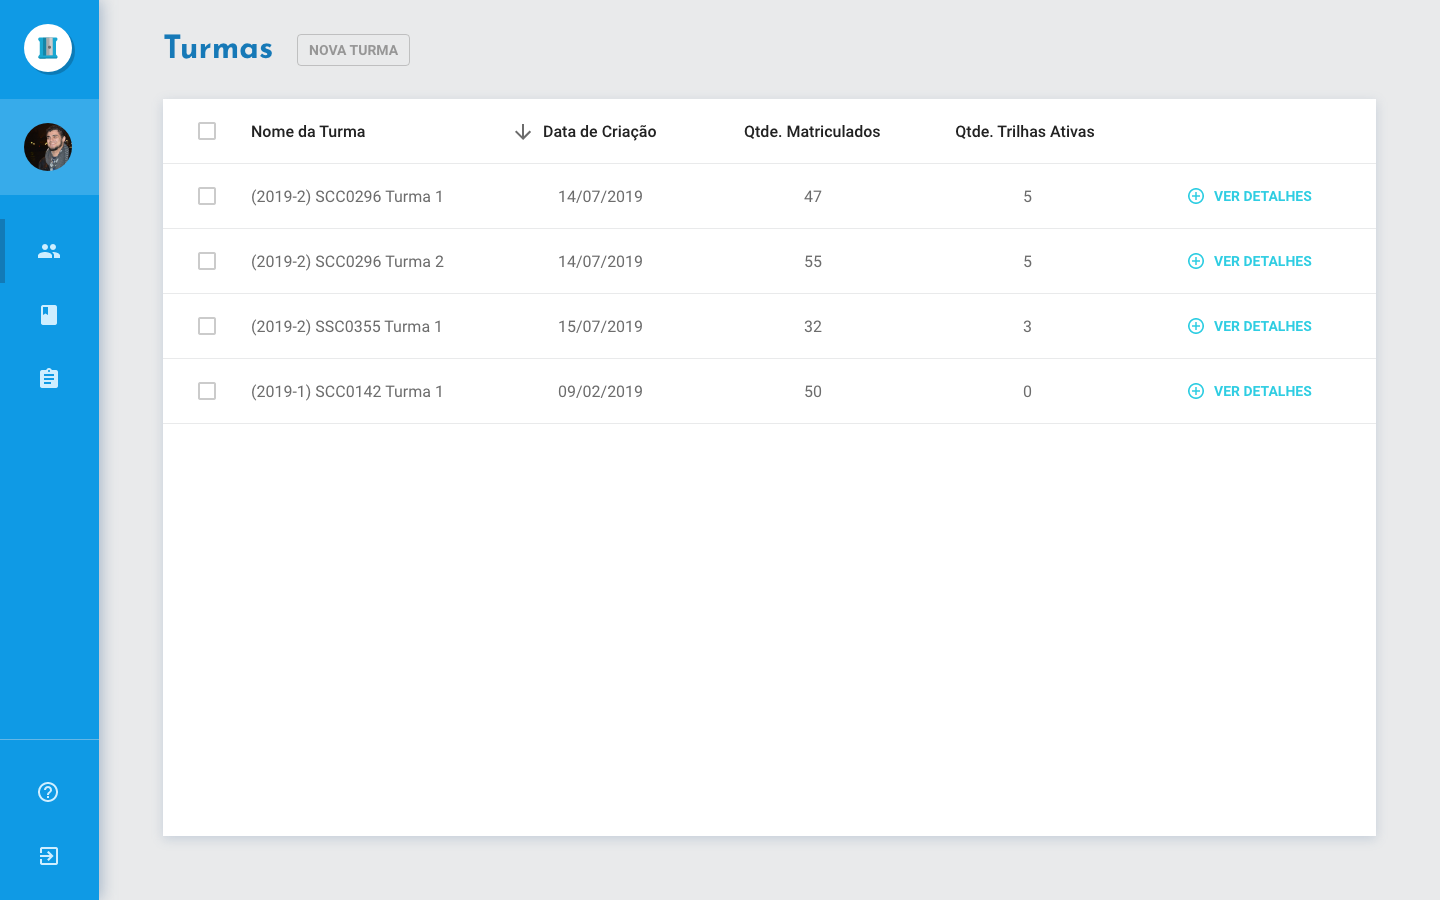
\includegraphics[width=\linewidth]{images/mocks/turma.png}
    \caption{Página de turmas da prova de conceito do sistema \emph{Sharpener}.}%
    \label{fig:turmas}
  \end{figure}

  \begin{figure}[htpb]
    \centering
    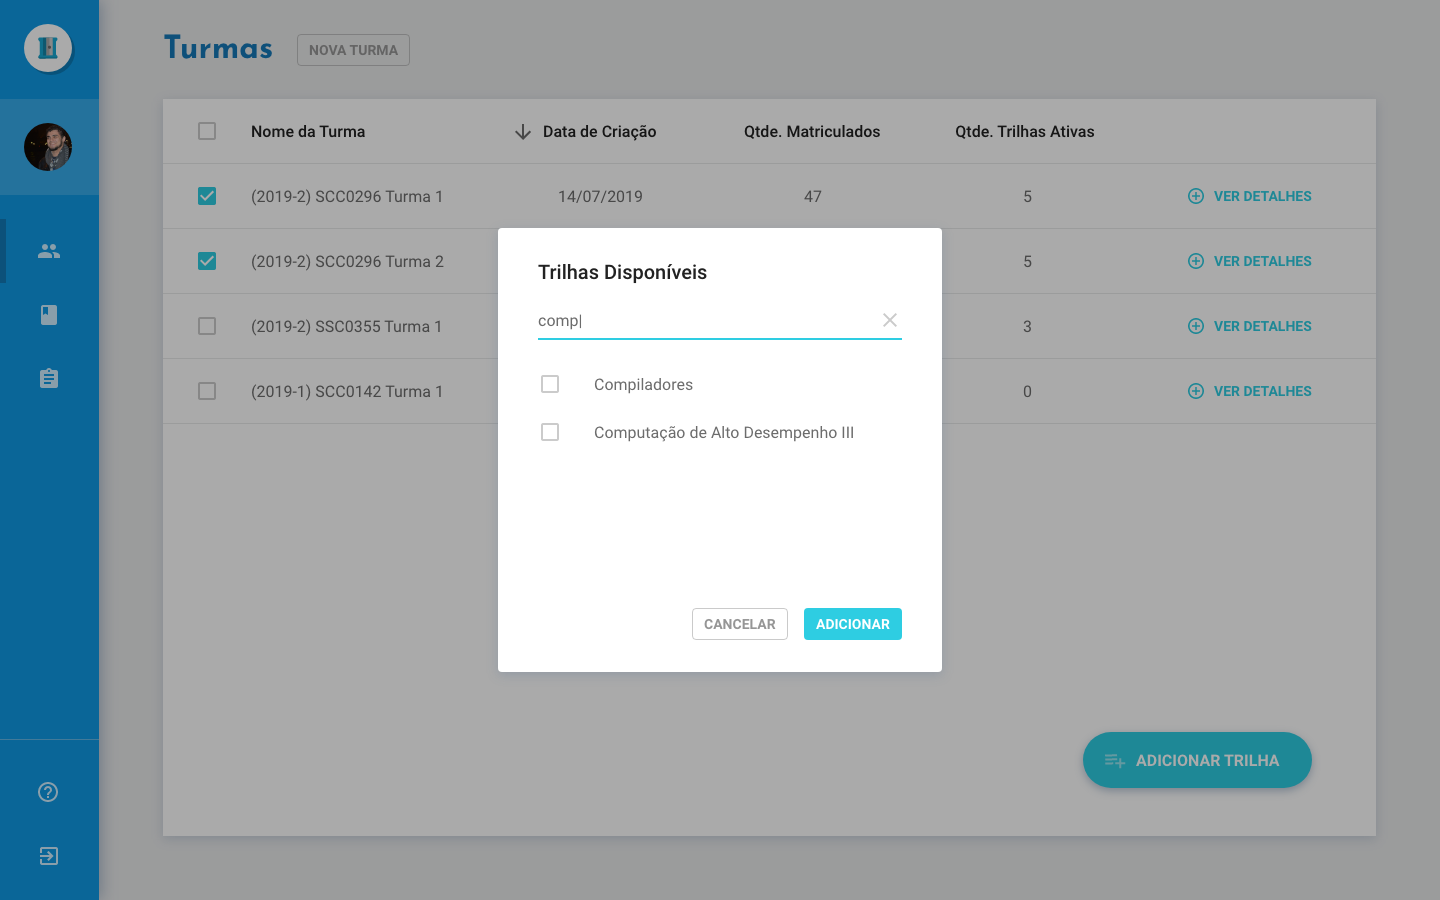
\includegraphics[width=\linewidth]{images/mocks/turmaAddTrackSearch.png}
    \caption{Página de turmas da prova de conceito do sistema \emph{Sharpener}, em 
	    que o professor inscreve suas turmas em trilhas.}%
    \label{fig:enroll_track}
  \end{figure}

  \begin{figure}[htpb]
  \centering
  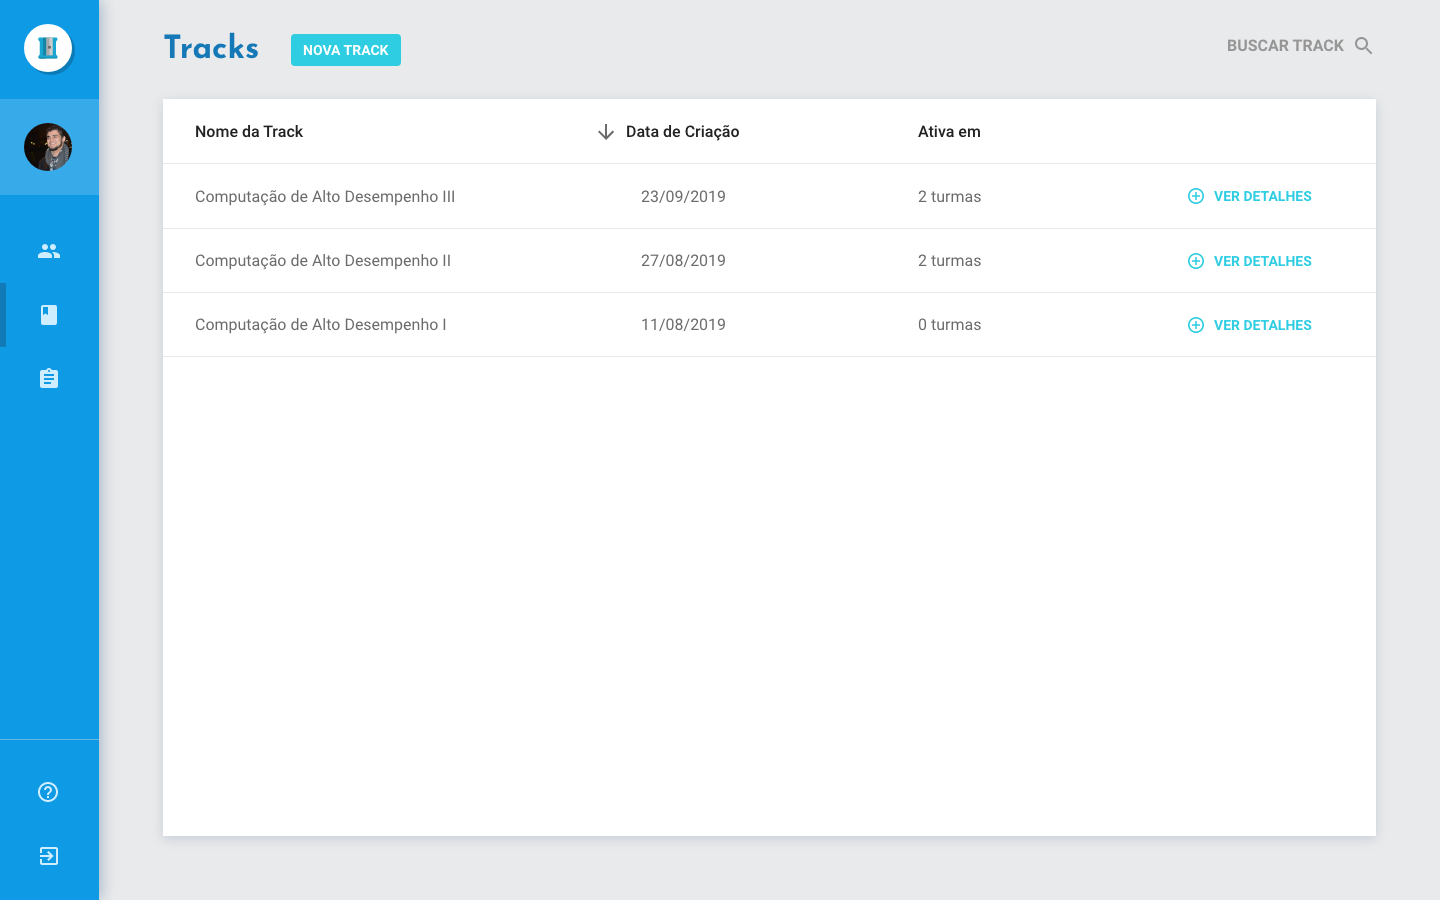
\includegraphics[width=\linewidth]{images/mocks/track.png}
  \caption{Página de trilhas da prova de conceito do sistema \emph{Sharpener}.}%
  \label{fig:track}
  \end{figure}

  \begin{figure}[htpb]
  \centering
  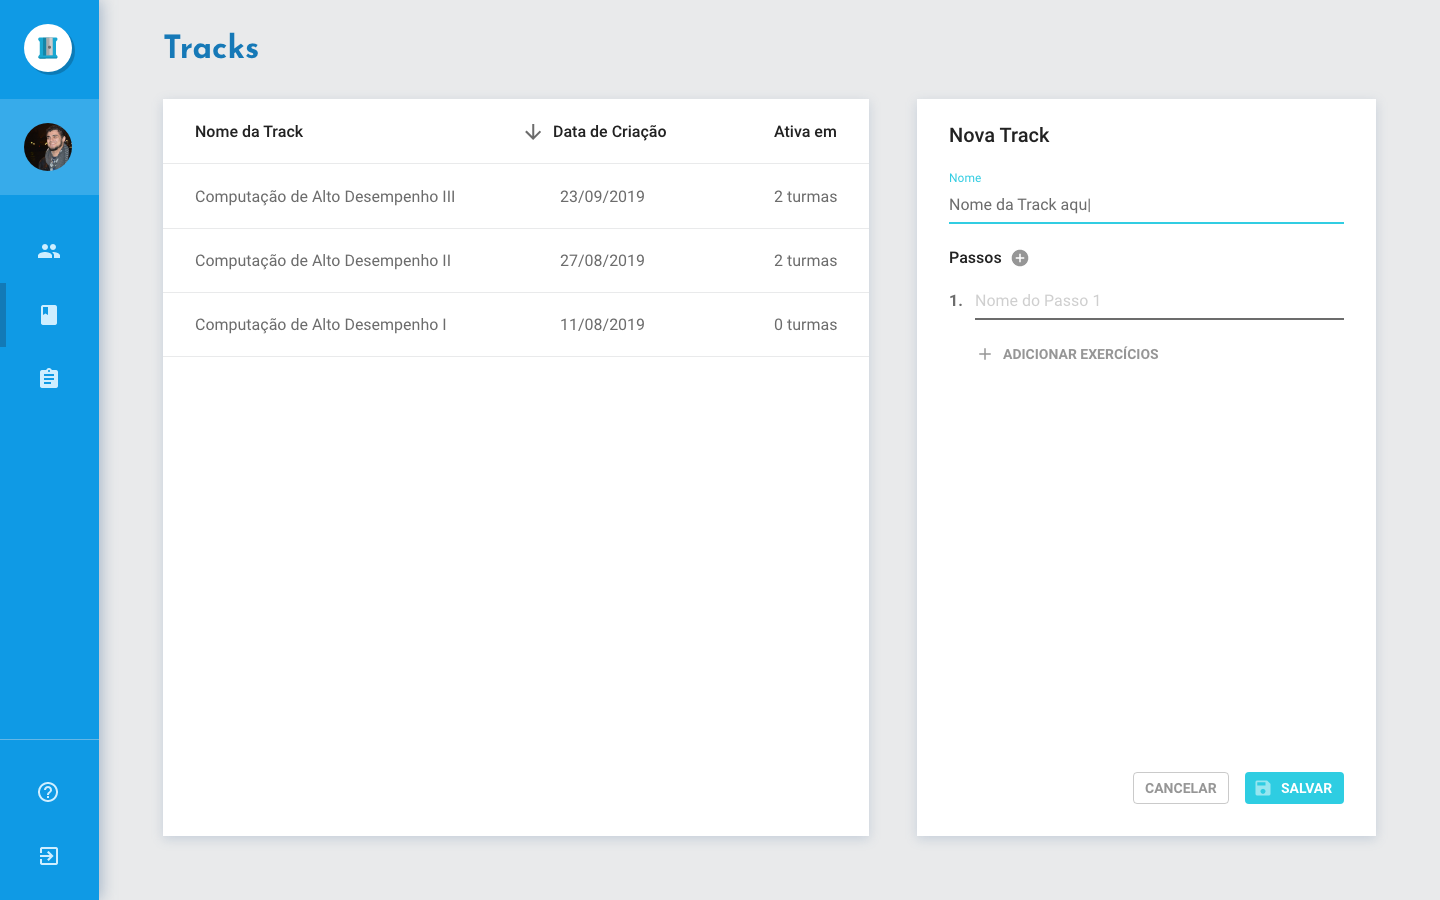
\includegraphics[width=\linewidth]{images/mocks/trackAdd1.png}
  \caption{Página de trilhas da prova de conceito do sistema \emph{Sharpener}, 
  em que uma nova trilha é criada.}%
  \label{fig:add_track1}
  \end{figure}

  \begin{figure}[htpb]
  \centering
  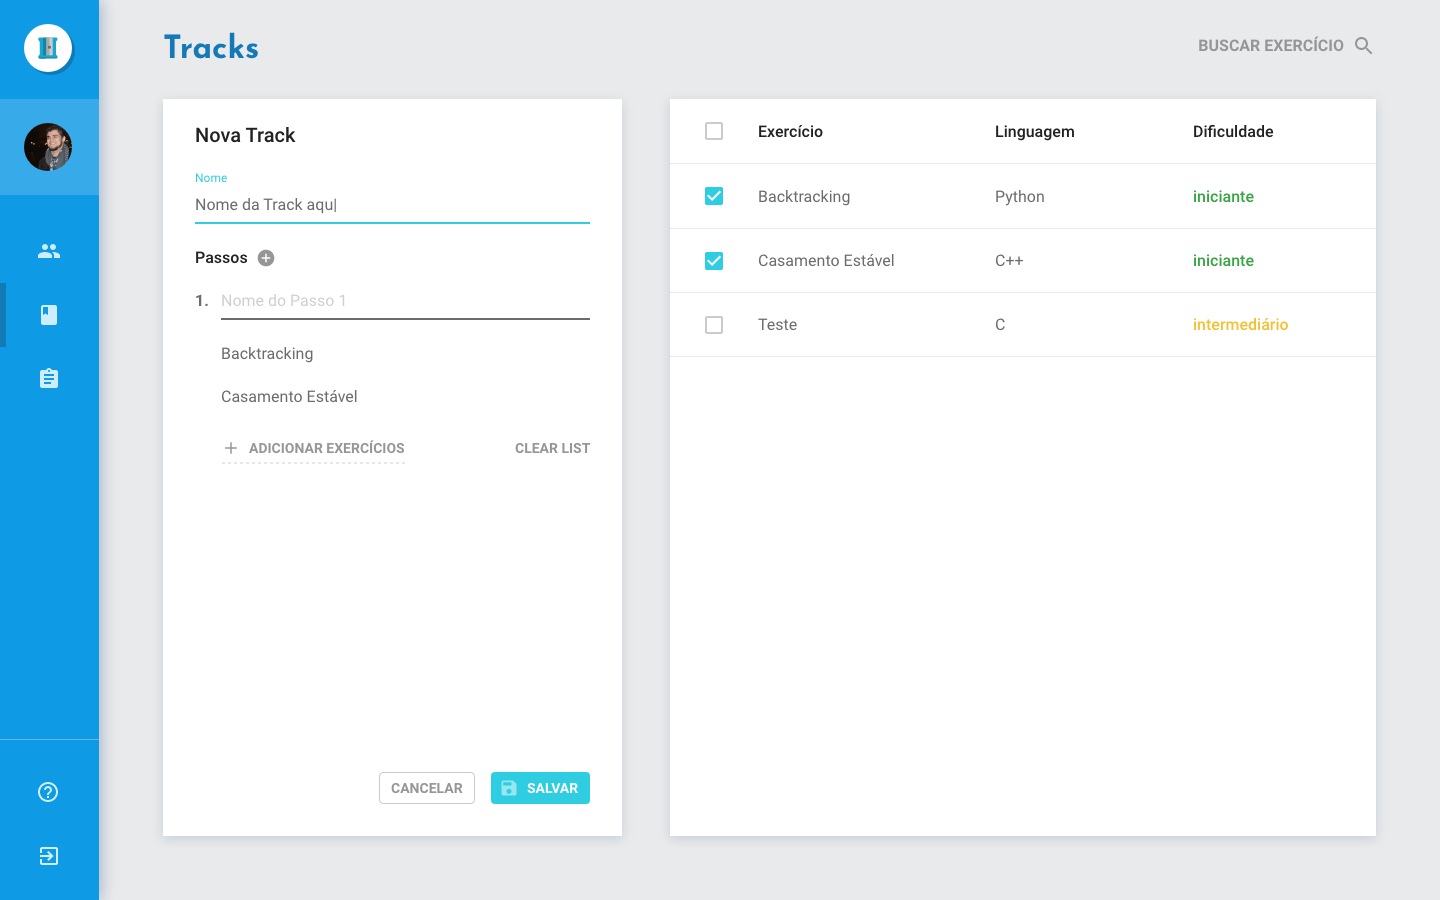
\includegraphics[width=\linewidth]{images/mocks/trackAdd4.png}
  \caption{Página de trilhas da prova de conceito do sistema \emph{Sharpener}, 
	  em que \emph{clusters de exercícios} são associados a passos de uma trilha.}%
  \label{fig:add_track4}
  \end{figure}

\begin{figure}[htpb]
  \centering
  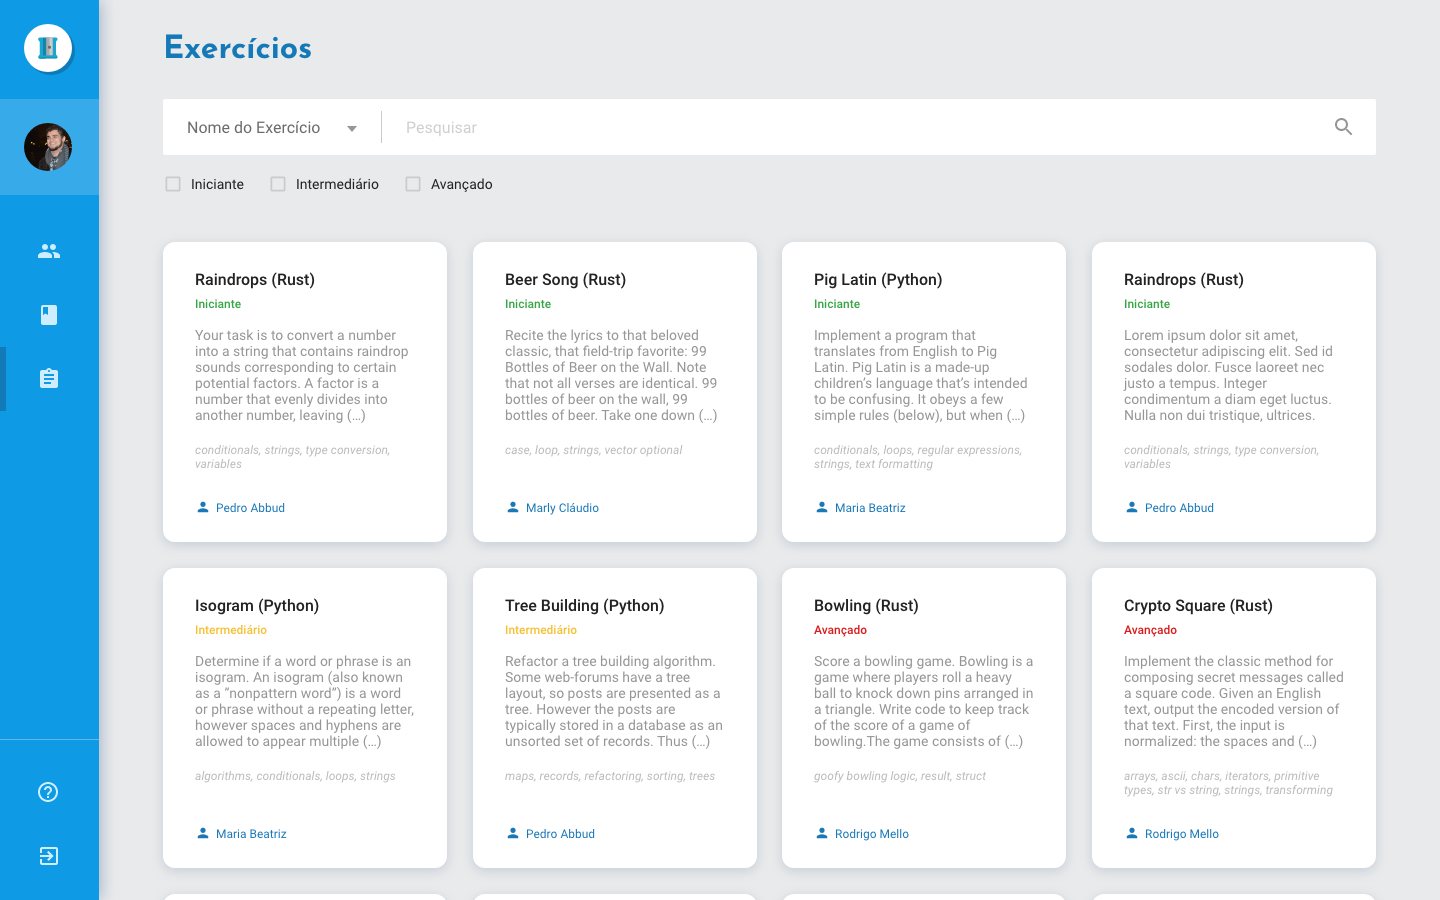
\includegraphics[width=\linewidth]{images/mocks/exercicios.png}
  \caption{Página de exercícios da prova de conceito do sistema \emph{Sharpener}.}%
  \label{fig:exercicios}
  \end{figure}
